\begin{figure}
\centering
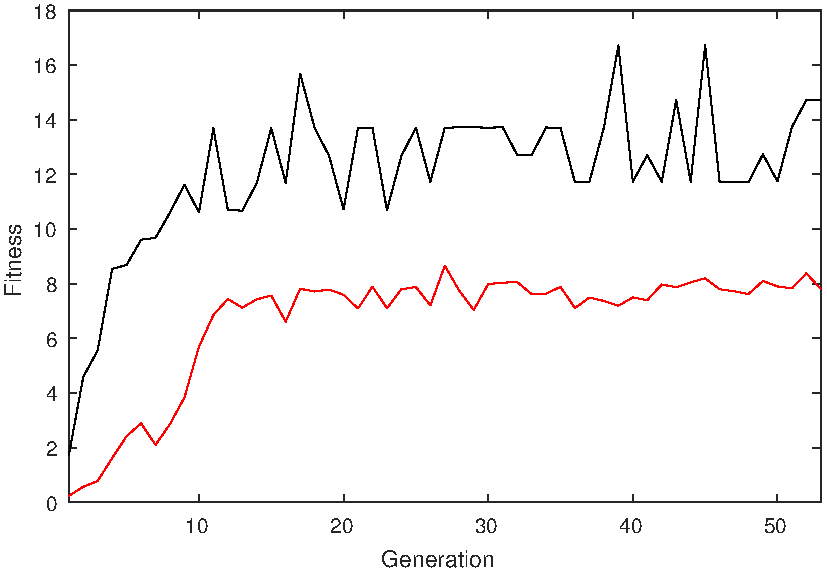
\includegraphics[width=.7\textwidth]{figs/fitness.pdf}
\caption{\label{fig:fitness} Black is best fitness in each generation and red is the average fitness in each generation. The energy available for each shark was 5000, the rest of the parameters is shown in Appendix \ref{app:param}}
\end{figure}

Despite the myriad of parameters used in the model, we were able to successfully train a shark that caught around 14 fish spending 5000 energy units. However, comparing this to the shark with the static algorithm, the shark with the static algorithm performed slightly better but with larger variance as can be seen in Table \ref{tab:fitness} 

This result does not suggest that this how the sharks brain work in reality.
\begin{table}
\centering
\begin{tabular}{r|c|c} 
Brain & Mean Fitness & Variance \\ \hline
ANN   &              &          \\ \hline
Algorithm &          &          \\ \hline
\end{tabular} 
\caption{\label{tab:fitness} Mean fitness values and variance over 25 trials with 5000 energy units in each trials for the ANN shark and the static algorithm shark.}
\end{table}
